%!TEX root = thesis.tex
\chapter{Implementation and Prototypes}
\label{chap:implementation}


This chapter documents the implementation of the benchmarking framework that was developed to evaluate the ingestion performance of InfluxDB, MongDB and TimescaleDB when storing time-series environmental observation data. The design of the implementation was intended to offer a controlled and reproducible environment where the three database systems could be subjected to identical workloads and then evaluated with a common set of performance metrics. The framework for benchmarking has a dataset management component, a database abstraction layer that’s implemented via repository classes, a component for benchmark execution responsible for workload timing and generation and a benchmark result repository used to store performance measurements. These components work together to ensure automated dataset loading, execution of ingestion workloads, collection of the performance measurements and the storage of benchmark results for subsequent analysis. 

To guarantee consistency across the different experiments, each database system was deployed inside a containerized environment using Docker. Separate repository implementations were created for MongoDB, TimescaleDB and InfluxDB to allow each database to be accessible through its native client while keeping a uniform benchmarking workflow. A dedicated benchmark database was also set up to persist benchmark results and facilitate later comparison and evaluation. The datasets used throughout the benchmark were created from synthetic environmental observation records representing time-series sensor measurements. Many dataset sizes were created to evaluate the way ingestion performance changes with an increase in data volume. The datasets were changes into appropriate formats for each database system while keeping the same underlying information content. This approach made sure that each database was evaluated with equivalent workloads. 

The implementation also has mechanisms for dataset loading, connection handling, benchmark configuration management, database initialization, throughput calculation, execution timing and result persistence. Special consideration was given to make the process repeatable by isolating benchmark runs, clearing data that was previously inserted and recording benchmark metadata alongside performance measurements. The rest of this chapter describes the architecture of the benchmarking framework, the preparation of the benchmark datasets, database environment configuration, the implementation of the benchmark execution workflow and the performance metrics that were collected during experimentation. The implementation details create the foundation for the evaluation and analysis presented in the next chapter. 



\section{System Architecture}

\subsection{Overall Benchmarking Framework}

To make sure that the comparison of MongoDB, TimescaleDB and InfluxDB is fair and repeatable, a unified benchmarking framework was created. The framework was intended to isolate the ingestion performance of the individual databases while making sure that all systems processed the same datasets under identical testing environments. Instead of creating different benchmarking implementations for each database, a common framework was used to standardize benchmark execution, data loading, result storage and performance measurement. The benchmarking framework consists of an orchestration layer, a database abstraction layer, the benchmark result storage layer and a data generation and loading pipeline. These components create a structured environment for running ingestion benchmarks and collecting performance metrics consistently across the evaluated database systems. 

\textbf{Benchmark orchestration layer :} 
This layer is the central control component of the framework. It does the job of coordinating the execution of benchmarking experiments. Dedicated benchmarking scripts were used for TimescaleDB, MongoDB and InfluxDB but all the scripts follow the same workflow for execution. For each benchmark run, the orchestration layer carries out the following tasks:

\begin{itemize}
    \item Loads the dataset metadata from the dataset size catalogue
    \item Loads the corresponding dataset from disk
    \item Sets up a connection to the target database
    \item Performs warm up operations specific to each database when required
    \item Runs ingestion operations with predefined batch sizes
    \item Measures execution time with high-resolution timers
    \item Calculates throughput metrics
    \item Stores the results from each benchmark in the BenchmarkDB repository
    \item Clears the target database before the next benchmark iteration
\end{itemize}

This design makes sure that all the database systems get evaluated with identical benchmark logic to reduce the possibility of implementation-specific bias influencing the results. 

\textbf{Database abstraction layer:}
This layer was implemented to provide a consistent interface for interacting with the different database technologies. Each system was represented by a dedicated repository class that included connection management, data insertion, querying and cleanup operation. The abstraction layer had a MongoDBRepo, InfluxDBRepo and TimescaleDBrepo. Each repository interacts with a different underlying database technology, but they expose similar functionality including:
\begin{itemize}
    \item Database connectivity verification via ping operations
    \item Single-record insertion methods
    \item Batch insertion methods
    \item Data cleanup and deletion operations
    \item Query execution functionality
\end{itemize}

This approach separates benchmark logic from details specific to database implementation. Because of this, modifications to database interaction mechanisms can be made independently without affecting the workflow for benchmark execution. For example, MongoDB batch insertion is run using the native insert\_manu() operation provided by its driver while TimescaleDB uses PostgresSQL’s execute\_values() mechanism and InfluxDB uses its batch write API. Despite these differences in implementation, all repositories offer a common interface for benchmark execution. 


\textbf{Benchmark result storage:}
A separate PostgresSQL database, BenchmarkDB, was created to store benchmark outputs independent of the databases being evaluated. Storing results externally helps prevent the benchmarking process from influencing the performance characteristics of the systems getting tested. BenchmarkDB is run using SQLAlchemy and has a dedicated table named ingestion\_benchmark\_results. Each execution creates a record with metadata about the experiment and the measured performance outcomes. The stored attributes were:

\begin{itemize}
    \item The name of the database system \& version
    \item Dataset identifier \& size
    \item Record count
    \item Insert batch size
    \item Total execution time
    \item Throughput in observations per second, bytes per second, kilobytes per second and megabytes per second
    \item Number of performed operations
\end{itemize}
A centralized benchmark repository helps make consistent storage possible, enables retrieval and supports the analysis of benchmark results across many experimental runs. 


\textbf{Data generation and loading pipeline:}
The benchmarking framework is based on a structured data generation and loading pipeline. Before benchmarking, datasets were generated and transformed into suitable formats for each target database system. The generated datasets were stored in different directories each corresponding to its database:
\begin{itemize}
    \item \texttt{Data/mongodb\_data/}
    \item \texttt{Data/influxdb\_data/}
    \item \texttt{Data/timescaledb\_data/}
\end{itemize}


MongoDB datasets were stored as JSON documents while TimescaleDB and InfluxDB datasets were stored as CSV files representing the different observations. In the benchmark execution, the framework loads the necessary dataset from disk, parses the data into the necessary in-memory representation and then passes the records to the corresponding repository for insertion. Dataset metadata like record count and storage size get loaded separately from the dataset\_sizes.csv file and are later used for throughput calculations. Separating metadata management, dataset storage and benchmark execution improves reproducibility and allows for the use of identical datasets across all database systems. 

Figure \ref{fig:benchmarking-framework} illustrates the overall architecture of the benchmarking framework: 

\begin{figure}
    \centering
    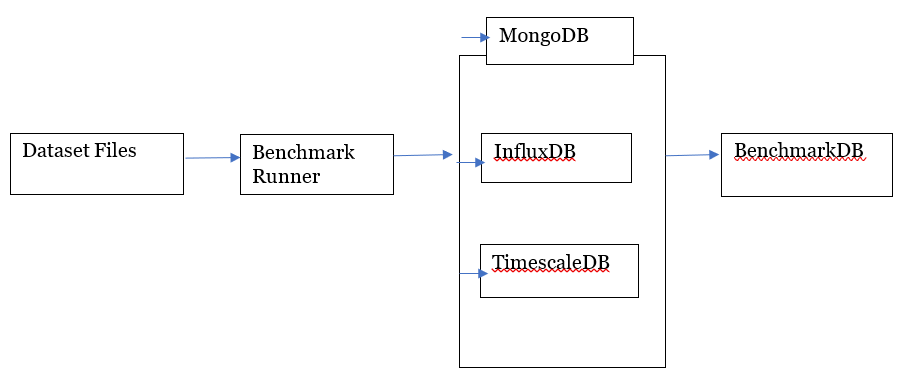
\includegraphics[width=0.8\textwidth]{figs/benchmarking_framework.png}
    \caption{Overall architecture of the benchmarking framework}
    \label{fig:benchmarking-framework}
\end{figure}

Inside of this architecture, the benchmark datasets get loaded by the benchmark runner which coordinates execution across the three database systems. Each database processes identical datasets under equivalent experimental conditions. The performance metrics collected in execution are subsequently stored in BenchmarkDB to be later analyzed and compared. 



\subsection{Project Structure}
The benchmarking framework was made into a modular project structure to improve reproducibility, maintainability and separation of concerns. Instead of placing all benchmarking logic in one codebase, functionality was divided into separate directories responsible for data storage, configuration management, result analysis, database interaction and thesis documentation. Only the directly relevant components to benchmark execution are discussed here. 

\textbf{Configuration directory (configs/):} 
This directory contains configuration files used to establish connections to the evaluated database systems and the benchmark result repository. Separate configs/ files are maintained for InfluxDB, MongoDB, TimescaleDB and BenchmarkDB. This approach helps the database connection parameters be modifiable without needing changes to the benchmark implementation. The configuration layer also betters portability by enabling the benchmarking framework to get deployed across different environments while keeping the benchmark logic consistent. 


\textbf{Data directory (data/):}
The data/ directory stores all used datasets during benchmarking. Separate subdirectories are kept for MongoDB, InfluxDB and TimescaleDB to accommodate the required data formats for each database system. Besides the benchmark datasets themselves, the directory had metadata files used to describe dataset characteristics like record counts and storage sizes. This metadata gets loaded during benchmark execution and is used to calculate throughput metrics and validate dataset consistency across experiments. The data directory works as the primary source of benchmark input data. 


\textbf{Source code directory (src/):}
This directory contains the implementation of the benchmarking framework. It includes repository classes, database clients, benchmark execution logic, logging utilities, configuration utilities and benchmark result management components. The source code is arranged according to database technology letting each database system maintain its own repository implementation while adhering to the common benchmarking workflow earlier described. The src/ directory is the core execution layer of the framework. 

\textbf{Notebook directory (notebooks/):}
The notebooks/ directory contains Jupyter notebooks used for exploratory data analysis, to validate benchmark outputs and to generate visualizations that are used in later chapters of this thesis. The separation of analytical notebooks from the benchmark execution code allows for experimental analysis to be performed without changing the underlying benchmarking framework. This contributes to reproducibility and supports iteration. all processed analytical outputs, figures and visualizations were generated and stored directly within the notebooks themselves.

\textbf{Thesis report directory (thesis-report/):}
This directory contains the supporting materials for the thesis and the manuscript for report preparation. Keeping the report inside the same project repository makes sure the benchmark implementations, figures, experimental results and documentation stay synchronized throughout the research process. The structure supports traceability between the implemented benchmarking framework and results presented in the final dissertation as well. 


\begin{figure}
    \centering
    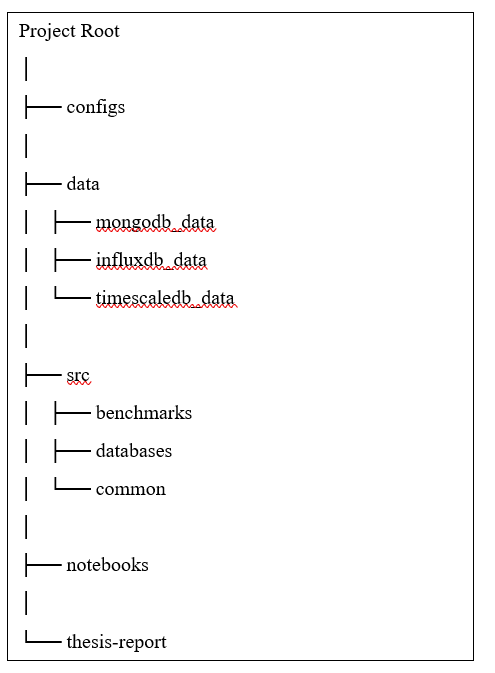
\includegraphics[width=0.8\textwidth]{figs/project structure.png}
    \caption{High-level project structure of the benchmarking framework}
    \label{fig:project-structure}
\end{figure}


\section{Benchmark Dataset Preparation}
\subsection{Observation Data Model}
The benchmarking experiments were run using a common observation data model representing marine sensor measurements. A standardized observation structure made sure that identical information is stored and processed by TimescaleDB, InfluxDB and MongoDB, enabling a fair comparison of ingestion performance across the database systems. Each observation represents one environmental measurement recorded by a sensor at a specific time and location. In addition to the measured value itself, the observation also has metadata describing the source of the measurement, the data quality indicators and the physical location where it was recorded. This structure reflects the characteristics of real-world ocean monitoring systems where sensor readings come accompanied by contextual information necessary for analysis and interpretation. 

The observation model has eleven fields which capture temporal information, sensor and node identifiers, geographical coordinates, quality assessment information and measurement details. Table~\ref{tab:observation-fields} presents the fields included in one observation record:


\begin{table}[h]
\centering
\begin{tabular}{|p{3cm}|p{6.5cm}|p{4.5cm}|}
\hline
\textbf{Field} & \textbf{Description} & \textbf{Example} \\
\hline
\texttt{sensor\_source} & Name of the sensor producing the measurement & Aanderaa temperature probe \\
\hline
\texttt{sensor\_source\_id} & Unique identifier of the sensor & sfi\_smart\_ocean;demo;d1;1 AANDERAA\_Temperature \\
\hline
\texttt{parameter} & Environmental parameter being measured & sea\_water\_temperature \\
\hline
\texttt{value} & Numerical value of the observation & 16.71 \\
\hline
\texttt{unit} & Measurement unit associated with the observation value & degrees\_C \\
\hline
\texttt{time} & Timestamp showing when the observation was recorded & 2025-06-01T12:00:00Z \\
\hline
\texttt{node\_source} & Name of the observation platform or monitoring node & Smart Ocean Node \\
\hline
\texttt{node\_source\_id} & Unique identifier of the monitoring node & sfi\_smart\_ocean;demo;d1;1 \\
\hline
\texttt{latitude} & Latitude coordinate of the observation location & 60.090717 \\
\hline
\texttt{longitude} & Longitude coordinate of the observation location & 5.263733 \\
\hline
\texttt{quality\_codes} & Quality control indicators describing the reliability of the observation & [0] \\
\hline
\end{tabular}
\caption{Observation data model}
\label{tab:observation-fields}
\end{table}


The timestamp field is the primary temporal attribute used to record the exact time when the measurement was collected. Because all evaluated databases support time-series data, this field is necessary for data organization and indexing. The longitude and latitude fields represent the geographical location of the observation. The coordinates allow measurements to get associated with specific monitoring sites and supports future spatial analysis. The node source identifier and node source fields describe the monitoring platform collecting the data. A monitoring node often hosts many sensors, making node-level metadata necessary for traceability and system management. 

Sensor source identifier and sensor source fields identify the specific sensors responsible for generating the measurement. They are included to allow observations from different sensor types to get stored inside the same dataset while maintaining source information. Unit, value and parameter fields together describe the measured environmental phenomenon. For example, a temperature sensor could produce a sea water temperature value expressed in degrees Celsius. Quality codes have data quality indicators used to assess reliability and validity of the observations. Such quality metadata is typically included in scientific and environmental monitoring systems to support downstream data analysis and validation. 


This observation model makes it possible to maintain a consistent benchmark dataset structure across influxDB, MongoDB and TimescaleDB. That way, all differences observed during benchmarking can be attributed to database behavior instead of variations in data representation. 

\subsection{Dataset Generation}
A series of synthetic environmental observation datasets was generated to evaluate database ingestion performance under varying workloads. The datasets were designed to conform to the observation model discussed in section 4.3.1 while offering controlled and repeatable benchmark inputs for the databases. Synthetic data was picked to make sure all benchmark experiments were done under identical conditions. Using generated observations helped to eliminate inconsistencies that come from missing values, irregular sampling intervals or different data quality commonly found in real world environmental monitoring datasets. The data also allowed the benchmark datasets size to be precisely controlled, making systematic evaluation of database performance across different data volumes possible. 


The raw synthetic observations were generated using JSON Generator \citep{jsongenerator}, a web-based tool that produces randomized data from a user-defined JavaScript template. This allowed the creation of realistic observation records with controllable field structures and value ranges, matching the schema required.


Generated observations represent environmental sensor measurements and include node, temporal, spatial, quality-control and sensor attributes. Once generated, the datasets were transformed into storage formats required by each target database system while preserving the underlying information content. Instead of benchmarking database performance using one dataset, a collection of progressively larger datasets was made. This approach makes it possible for ingestion performance to be evaluated under increasing workloads and enables the observation of how the database system scales as the volume of incoming data grows. Sixteen benchmark datasets were generated, ranging from very small datasets with five observations to larger ones with fifty thousand observations. The associated storage requirements and dataset sizes were recorded in the dataset\_sizes.csv metadata file and used in benchmark execution to calculate throughput metrics. Table~\ref{tab:batch-sizes} presents the benchmark datasets used throughout the study:


\begin{table}[h]
\centering
\begin{tabular}{|r|l|r|r|r|r|}
\hline
\textbf{Batch ID} & \textbf{Dataset Name} & \textbf{Observations} & \textbf{Size (Bytes)} & \textbf{Size (KB)} & \textbf{Size (MB)} \\
\hline
1  & \texttt{batch\_1\_5\_obs}      & 5      & 1,071      & 1.05     & 0.001 \\
\hline
2  & \texttt{batch\_2\_10\_obs}     & 10     & 2,141      & 2.09     & 0.002 \\
\hline
3  & \texttt{batch\_3\_25\_obs}     & 25     & 5,349      & 5.22     & 0.005 \\
\hline
4  & \texttt{batch\_4\_50\_obs}     & 50     & 10,692     & 10.44    & 0.010 \\
\hline
5  & \texttt{batch\_5\_100\_obs}    & 100    & 21,385     & 20.88    & 0.020 \\
\hline
6  & \texttt{batch\_6\_250\_obs}    & 250    & 53,459     & 52.21    & 0.051 \\
\hline
7  & \texttt{batch\_7\_500\_obs}    & 500    & 106,924    & 104.42   & 0.102 \\
\hline
8  & \texttt{batch\_8\_1000\_obs}   & 1,000  & 213,835    & 208.82   & 0.204 \\
\hline
9  & \texttt{batch\_9\_2000\_obs}   & 2,000  & 427,720    & 417.70   & 0.408 \\
\hline
10 & \texttt{batch\_10\_3000\_obs}  & 3,000  & 641,522    & 626.49   & 0.612 \\
\hline
11 & \texttt{batch\_11\_5000\_obs}  & 5,000  & 1,069,189  & 1,044.13 & 1.020 \\
\hline
12 & \texttt{batch\_12\_7500\_obs}  & 7,500  & 1,603,854  & 1,566.26 & 1.530 \\
\hline
13 & \texttt{batch\_13\_10000\_obs} & 10,000 & 2,138,394  & 2,088.28 & 2.039 \\
\hline
14 & \texttt{batch\_14\_20000\_obs} & 20,000 & 4,276,864  & 4,176.62 & 4.079 \\
\hline
15 & \texttt{batch\_15\_30000\_obs} & 30,000 & 6,415,152  & 6,264.80 & 6.118 \\
\hline
16 & \texttt{batch\_16\_50000\_obs} & 50,000 & 10,691,719 & 10,441.13 & 10.196 \\
\hline
\end{tabular}
\caption{Benchmark database sizes}
\label{tab:batch-sizes}
\end{table}


Progressively larger datasets were used for a number of reasons. First, they help the evaluation of ingestion performance across a wide range of workload sizes. Small datasets offer insight into system behavior during low-volume ingestion scenarios while larger datasets simulate operational environments that are more demanding. Secondly, increasing dataset sizes enable the investigation of scalability characteristics. A database could perform efficiently while processing hundreds of observations but show reduced throughput with the increase in the volume of incoming data. Using many dataset sizes provides a more complete understanding of performance behavior than a single benchmark dataset. Dataset progression also makes it possible to identify potential bottlenecks related to storage management, write operations, buffering mechanisms, transaction handling and indexing overhead. These effects only become visible as the dataset size grows. Finally, standardized datasets ensure that all the evaluated databases are evaluated through identical workloads. This consistency is necessary to achieve fairness.



\subsection{Database-specific dataset formats}
Even though the benchmark used the same environmental observation data across the different database systems, the dataset was represented differently to match database storage models. The data structures were made according to the recommended data modeling approach for each database while keeping the same underlying information content. 

\textbf{MongoDB dataset format:}
MongoDB stores data as JSON-like BSON documents. Here, each document represented a measurement event from an ocean monitoring node at a specific point in time. A document had:
\begin{itemize}
    \item Node information
    \item Geographic location
    \item Timestamp
    \item Different sensor observations
\end{itemize}

Individual sensor observations had a value, unit, parameter name and quality code. The dataset structure made it possible to embed many related observations inside one document, reducing the number of write operations necessary during ingestion. Table 

Each sensor observation contained a parameter name, value, unit and quality code. The dataset structure allowed multiple related observations to be embedded within a single document, reducing the number of write operations required during ingestion. Table~\ref{tab:mongodb-document-structure}  presents the structure of a MongoDB document. (In the benchmark dataset, each MongoDB document contained five sensor observations collected from the same monitoring node and timestamp.)

\begin{table}[h]
\centering
\begin{tabular}{|l|p{8cm}|}
\hline
\textbf{Field} & \textbf{Description} \\
\hline
\texttt{source} & Monitoring node name \\
\hline
\texttt{source\_id} & Unique node identifier \\
\hline
\texttt{location} & Geographic coordinates \\
\hline
\texttt{time} & Observation timestamp \\
\hline
\texttt{observations} & Array of sensor observations \\
\hline
\texttt{meta} & Additional node metadata \\
\hline
\end{tabular}
\caption{Structure of a MongoDB Document}
\label{tab:mongodb-document-structure}
\end{table}



\textbf{TimescaleDB dataset format:}
TimescaleDB stores information using a relational table structure. Because of this, each environmental observation was represented as a separate row. The dataset was stored in a table containing spatial, temporal and sensor measurement attributes. This structure produced one database row for every individual sensor measurement appearing as shown in Table~\ref{tab:timescaledb-format} below:

\begin{table}[h]
\centering
\begin{tabular}{|l|l|r|l|}
\hline
\textbf{time} & \textbf{parameter} & \textbf{value} & \textbf{unit} \\
\hline
2025-01-01 00:00:00 & sea\_water\_temperature & 18.68  & degrees\_C \\
\hline
2025-01-01 00:00:00 & sea\_water\_salinity    & 35.45  & PSU \\
\hline
2025-01-01 00:00:00 & dissolved\_oxygen       & 155.80 & umol L-1 \\
\hline
\end{tabular}
\caption{An example representation for TimescaleDB}
\label{tab:timescaledb-format}
\end{table}



\textbf{InfluxDB dataset format:}
Typically, influxDB stores time-series data as measurements with fields, tags and timestamps. Before insertion, observations from the dataset were converted into observation objects and then changed into InfluxDB point objects. Within the implementation, these attributes, node\_source, node\_source\_id, sensor\_source, parameter and unit were stored as tags. Value, longitude, latitude and quality\_codes were stored as fields. Each point was written to the measurement called ocean\_observations using precise timestamps to the nanosecond. Figure \ref{fig:influxdb-record} is a conceptual representation of the record:

\begin{figure}
    \centering
    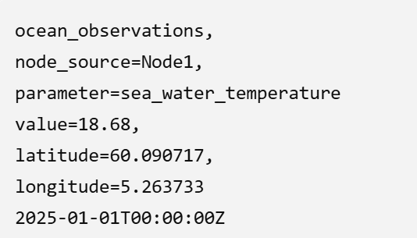
\includegraphics[width=0.8\textwidth]{figs/InfluxDB_record.png}
    \caption{Conceptual representation of an InfluxDB record}
    \label{fig:influxdb-record}
\end{figure}

The use of fields and tags enables InfluxDB to optimize retrieval and indexing of time-series measurements while maintaining efficient storage of sensor values. 
While all three database systems stored identical environmental information, their internal representation was different. MongoDB grouped many sensor observations into one document, TimescaleDB stored observations like individual relational records and influxDB converted observations into time-series points with timestamps, tags and fields. The differences reflect the underlying design philosophy for each database system and are expected to influence ingestion performance during benchmarking. 



\section{Database Environment Configuration}
\subsection{Containerized deployment}
To make benchmarking repeatable and fair, all database systems were deployed with docker containers orchestrated via Docker Compose. Containerization was done to offer a standardized execution environment in which all the databases could be configured, started and managed consistently across benchmark runs. Docker Compose was used to defined and coordinate the necessary services via declarative configuration files. Instead of installing each database directly on the host OS, every database instance was executed inside its own isolated container. This approach made sure that the benchmark framework interacted with individual databases through a controlled and reproducible environment. The decision to use a container was motivated by three considerations – reproducibility, isolation and environmental consistency. 

A key objective of benchmarking is the ability to reproduce experimental results. Docker Compose makes it possible to define infrastructure configurations as code which means that the same database versions, service configurations and network settings can be recreated when the benchmark is executed. This approach lowers variability introduced by manual procedures for installation and allows future researchers to recreate the benchmarking environment with little configuration effort. Maintaining database configurations inside version-controlled deployment files keeps the experimental setup repeatable and transparent. 

The different database systems were deployed inside independent containers. The separation prevented software dependencies, runtime configurations and libraries from interfering with one another. Isolation was especially necessary because TimescaleDB, MongoDB and InfluxDB, all employ different communication protocols, storage engines and runtime requirements. Containerization made sure that each database operated inside its intended environment while staying accessible to the benchmarking framework via defined network interfaces. Isolated containers also made maintenance tasks like clearing datasets, restarting services and resetting experimental conditions between benchmark runs possible. 



Variations in operating system configurations, dependency management and software versions can all influence benchmarking results. Docker Compose helped to minimize the sources of variation by making sure that all benchmark executions used the same container images and runtime configurations. As a result, differences observed during benchmarking were more likely to reflect the characteristics of the database systems instead of inconsistencies in the surrounding execution environment. This contributes to the internal validity of the experiments and adds to the reliability of the performance measurements obtained. Figure \ref{fig:cdd-Architecture} illustrated the containerized deployment architecture that was used during benchmarking.

The use of containers provided a stable and reproducible foundation for executing ingestion benchmarks across the database systems while keeping the experimental conditions consistent throughout the study.







\begin{figure}
    \centering
    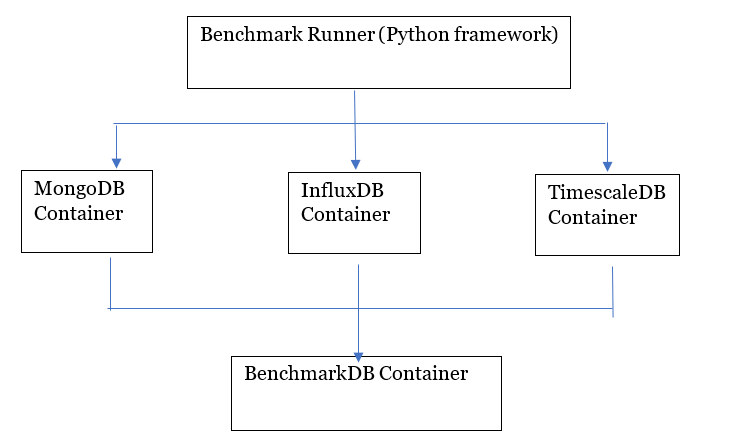
\includegraphics[width=0.8\textwidth]{figs/cdd_Architecture.png}
    \caption{Containerized Database Deployment Architecture}
    \label{fig:cdd-Architecture}
\end{figure}



\subsection{MongoDB Configuration}
MongoDB was deployed in a container within the Docker Compose environment. The configuration was intended to provide an isolated and reproducible deployment while making sure that database initialization and access control were automatically established at system startup. The benchmark used the official MongoDB docker image specified in the Docker Compose configuration as:
\begin{verbatim}
mongodb:
    image: mongo:8
\end{verbatim}
The official image was used to ensure consistency across executions and provide a standardized environment without needing manual installation on the host machine. The container exposed MongoDB’s default service port (27017), which was mapped to a configurable host port via environment variables. This way, the benchmarking framework could communicate with the database using consistent network interface no matter the host environment. 

Authentication was enabled via environment variables supplied at container initialization. The MongoDB root username and password were created automatically at the first launch of the container.

Environment variables helped to separate sensitive credentials from source code and configuration files while letting different deployment environments use independent authentication settings. This approach aligns with standard container security practices and made sure that benchmark operations were run against an authenticated database instance. 

The database was configured to run initialization scripts automatically at startup via the Docker entrypoint initialization mechanism. 

\begin{verbatim}
volumes:
  - mongo\_data:/data/db
  - ./init-mongo:/docker-entrypoint-initdb.d:ro
\end{verbatim}


The init-mongo directory was mounted as a read-only volume and provided initialization scripts executed when the container was created. The idea here was to enable the automatic preparation of the benchmark database environment without needing manual intervention after deployment. Automating initialization meant that the benchmark could recreate the database environment consistently across different experimental runs. 

A dedicated Docker volume was attached to the MongoDB container:

\begin{verbatim}
volumes:
  - mongo\_data:/data/db
\end{verbatim}

The volume persisted MongoDB files independently of the lifecycle of the container. It made sure that benchmark data stayed available even if the container was recreated or restarted. Persistent storage also made repeated benchmark executions and result verification possible.

To make sure the database was available before execution, a container health check was set up:

\begin{verbatim}
healthcheck:
  test: ["CMD", "mongosh", "--eval", "db.adminCommand('ping')"]
\end{verbatim}

Periodically, the health check sent a ping command to the MongoDB server to verify that the database was ready to accept connections. This helped lower the risk of benchmark execution starting before the database service was fully initialized. 

\subsection{TimescaleDB Configuration}
Timescale was the relational time-series database platform used in this study. Its system was also configured using a Docker container but based on PostgreSQL 17 with its extension pre-installed. The reason for the configuration was to benefit from the database’s traditional relational functionality but also be able to make optimizations to manage large volumes of data. The TimescaleDB service was deployed with the official image:
\begin{verbatim}
timescaledb:
  image: timescale/timescaledb:latest-pg17
\end{verbatim}

The image combines the PostgreSQL relational database engine with TimescaleDB extension to make it possible to integrate time-series capabilities directly into a standard SQL database environment. Database creation parameters and authentication credentials were supplied via environment variables during container initialization.

PostgreSQL as the underlying platform allowed the benchmark framework to interact with the TimescaleDB via standard SQL operations while benefiting from PostgreSQL’s mature transaction management, query processing capabilities and indexing mechanisms. The database extends PostgreSQL by introducing optimization mechanisms and data structures specifically designed for time-series workloads. Instead of replacing PostgreSQL functionality, the extension adds specialized support for handling timestamped observations. In the benchmark implementation, environmental observations got stored in a relational table named observations. Each observation was represented as a single database record with spatial, temporal and sensor-related attributes. The repository implementation interacted with TimescaleDB with batch insertion operations and SQL queries. Large ingestion workloads were run using execute\_values() function supplied by the PostgreSQL driver.

A basic feature of TimescaleDB is the hypertable. It shows up to users as a normal PostgreSQL table, but internally, it is partitioned into smaller chunks by time interval. This architecture makes storage efficient and supports querying and indexing of large time-series datasets. In the benchmark environment, the observations table was the primary storage structure for environmental sensor data. During initialization, the table was converted into a hypertable using TimescaleDB’s hypertable creation functionality. The time attribute of each observation became the partitioning dimension, allowing records to get organized according to their timestamps. This design supports efficiency and optimizes the retrieval of historical data over specific time ranges. 

From the perspective of the benchmarking application, data insertion happened via a single logical table. However, internally, TimescaleDB distributed records across many chunks according to their timestamp, enabling scalability. Database initialization scripts were added into the container at startup:


\begin{verbatim}
volumes:
  - timescale\_data:/var/lib/postgresql/data
  - ./init-timescaledb:/docker-entrypoint-initdb.d
\end{verbatim}
The initialization directory allowed database schema creation and TimescaleDB configuration tasks to be executed automatically when the container was first deployed. Persistent storage was provided through the timescale\_data Docker volume, to make it possible for benchmark data to be available across container restarts. A health check was configured before execution to verify service availability. 



\subsection{InfluxDB Configuration}
InfluxDB was run using its official Docker image as part of the containerized benchmarking environment. The database was automatically configured at startup using environment variables defined in the Docker Compose configuration to make sure that the database could be consistently recreated across different benchmark executions without needing manual setup. InfluxDB differs from traditional relational databases in how it organizes data in buckets and organizations. An organization provides logical grouping for the resources in the database while the bucket works as the primary storage container for time-series records. At initialization, a dedicated bucket and organization were made to store the benchmark datasets used in the study. Authentication was implemented with the token-based security mechanism offered by InfluxDB 2.7. During startup, an access token was auto-generated and supplied to the benchmark application via environment variables. This token was used by the Python repository layer for authentication of all query operations and data ingestion. Token-based authentication made access control simpler while securing communication between the database instance and benchmark framework. 



\subsection{Benchmark Database}
Besides the three databases under evaluation, a separate PostgresSQL database was deployed to be the benchmark result repository – BenchmarkDB. It was not included in the performance comparison itself. Its purpose was to create a centralized location to store benchmark execution results generated in the experiments. BenchmarkDB was implemented using PostgresSQL 17 and run as an independent Docker container inside the benchmarking environment. A dedicated data model, IngestionBenchmarkResult, was created to capture performance metrics generated during each execution. The stored information included the dataset identifier, database system under test, batch size, data size, record count, execution time, timestamp of the benchmark execution and throughput measurements. 

The benchmark framework inserted results into BenchmarkDB after the completion of each run. This made sure that performance measurements were independently preserved and could be retrieved for subsequent visualization and analysis. The benchmark results were separated to create a consistent and reliable mechanism for collecting experimental data. The stored results were used for visualization, statistical analysis and comparison of database ingestion performance. 



\section{Benchmark Framework Implementation}
\subsection{Configuration Management }
A reproducible and flexible configuration management approach was implemented to separate deployment-specific settings from application logic. The benchmark framework used YAML config files alongside environment variables to manage storage locations, database connection parameters, logging settings, and other runtime operations. This allowed the execution of the same codebase across different environments without needing to modify the source code. 

Application configuration was stored in YAML files inside the project’s configuration directory. Each database system maintained its own configuration file with parameters relevant to the specific technology. The YAML structure separated configuration into logical sections. The general section contains application-level settings like dataset paths and log file locations while the database section has connection parameters needed to establish communication with the database instance. This organization simplifies maintenance as the system grows and improves readability. Using separate config files per database also lowered coupling between benchmark components. It allowed the modification of database-specific settings without affecting other parts of the framework. 


Instead of storing sensitive information in the configuration files directly, the framework used environment variables to provide deployment-specific values and credentials. Passwords, ports, database usernames, hostnames, authentication tokens and other parameters were added to the configuration files during startup. This served three purposes; first, sensitive credentials were not added to source code repositories which lowers the risk of accidental disclosure. Second, the same file could be reused across multiple environments like testing, production deployments and development. The only thing needed to change is the environments variable values. Finally, the approach naturally aligned with the Docker-based deployment strategy applied all through the benchmarking framework. Environment variables that were defined in Docker compose could be consumed by the benchmarking application without needing to change. 

Configuration loading was done through the load\_config() function stored in src/common/config.py. The job of this function was to be the entry point for reading and processing configuration files. The loading process consisted of validating the configuration file path, rendering template variables with Jinja2, resolving environment variable references and parsing the resulting YAML document. Additionally, the configuration framework had a built-in validation logic through the env\_var() helper function to retrieve environment variable values and verify that required variables were there before application execution could proceed. The idea of the validation mechanism was to prevent benchmark executions from beginning with incomplete config settings. Missing authentication tokens, hostnames or credentials were immediately detected during the startup of the application instead of causing failures during benchmark execution. Early validation is especially important in automated benchmarking environments whose experiments run for long and generate large volumes of performance data. 

Even though configuration files had a common structure, each database system had its own configuration definition to enable the framework to accommodate different requirements from each database. For example, InfluxDB needed authentication tokens, organization identifiers and bucket names while TimescaleDB needed PostgreSQL connection parameters, user credentials and database names. For reproducibility, all database parameters, authentication settings, storage locations and logging paths were defined explicitly outside the source code and then dynamically loaded at runtime.

\subsection{Repository Pattern}
The benchmarking framework adopted the repository pattern as an abstraction layer between the benchmark execution logic and the database implementations underneath it. This design made it possible for benchmark routines to interact with the databases through consistent operations while isolating database-specific details inside dedicated repository classes. Each repository encapsulated query execution, connection management, data deletion procedures and data insertion as required by each database system. A primary objective of the framework for benchmarking was to compare database performance, not just differences in application implementation. To make this possible, benchmark logic needed to be independent of database-specific APIs and query languages. Without the abstraction layer, the benchmark runner would need different implementations for the different databases, creating code duplicates and making it hard to ensure consistency across all systems. 

\textbf{MongoDB Repository:}
MongoDB functionality was run through the MongoDBRepo class which extends the MongoDBClient. It provides methods to connect the database, query data, insert documents, manage collections, delete records and perform aggregations. During benchmark execution, collection and database references are retrieved once and stored in memory before timing starts via the connect\_and\_cache() feature. This helps to reduce Python-side overhead and makes sure that the measured execution time reflects database operations instead of connection management activities. Since MongoDB stores data in the form of JSON-like documents, the repository handles these operations directly via the MongoDB driver while hiding implementation details. 

\textbf{InfluxDB Repository:}
The functionality for InfluxDB was implemented through InfluxRepo. The class performed an extra transformational step where observation objects are converted into Point objects before insertion. The conversion was implemented through \_to\_point() which mapped observation attributes to timestamps, fields and tags. Insertion performance gets measured immediately around the write operation using time.perf\_counter\_ns(). 


\textbf{TimescaleDB Repository:}
Since TimescaleDB is built on PostgreSQL, observations are stored in a relational table. The repository translates observation objects into SQL-compatible tuples before running insert statements. This implementation supports both batch insertion and single-record operations. Batch insertion is done with PostgreSQL’s execute\_values() function that allows the insertion of many rows through one SQL statement. Insertion times are measured with high-resolution timers to support precision. 

While each repository interacts with different database models, all implementations expose a similar set of capabilities that were needed by the benchmarking framework including batch insertion, database connection, execution time managements and connectivity testing. The repository pattern played a major role in ensuring maintainability and fairness inside the benchmarking framework. 


\subsection{Data Loading Mechanism}
The mechanism for locating datasets, loading them into memory and retrieving metadata before execution needed to be consistent. Because the study evaluated database systems using varied datasets, a standardized data loading process was implemented to make sure all databases were benchmarked with equivalent input data. The datasets were stored in database-specific directories arranged by batch size. During execution, the benchmark runner identified the dataset based on its name and selected batch identifier. Dataset naming convention also included the number of observations per dataset. For example, a dataset named batch\_8\_1000\_obs represented the eighth benchmark dataset and contained 1,000 observations. This was done for simplicity and to reduce the risk of loading files incorrectly. Besides loading the dataset, the framework also loaded metadata describing characteristics for each dataset. This was stored in a dataset\_sizes.csv file that ensured the dataset size measurements stayed consistent across all benchmark executions. 

\subsection{Benchmark Result Model}
All benchmark outcomes get stored in the IngestionBenchmarkResult model which is the central repository for performance measurements from experimental execution. Each benchmark run produces a result record with metadata about the scenario, dataset used, target database system and performance metrics obtained. The model captures the time elapsed, dataset characteristics, throughput metrics, benchmark configuration parameters and operational metrics like the number of performed inserts. 

\section{Ingestion Benchmark Implementation}
The ingestion benchmarking framework was designed to evaluate the write performance of the databases under increasing data volumes. While each database needed a different ingestion implementation because of differences in data models and client APIs, all benchmarks used a common workflow to make sure the results were comparable and consistent. For each run, the appropriate dataset was loaded from the data directory and its metadata was retrieved. The benchmark then connected to the target database and ran a series of warm-up operations before recording any measurements. After the warm-up phase, the benchmark ran database-specific insertion processes while measuring execution time with high-resolution timers. Once insertion was complete, throughput metrics were calculated and the results stored in BenchmarkDBRepo. Finally, the data inserted was removed from the database to make sure the next execution begun from a consistent and clean state. 

Figure \ref{fig:ingestion-benchmark-workflow} illustrates the overall architecture of the benchmarking framework: 
\begin{figure}
    \centering
    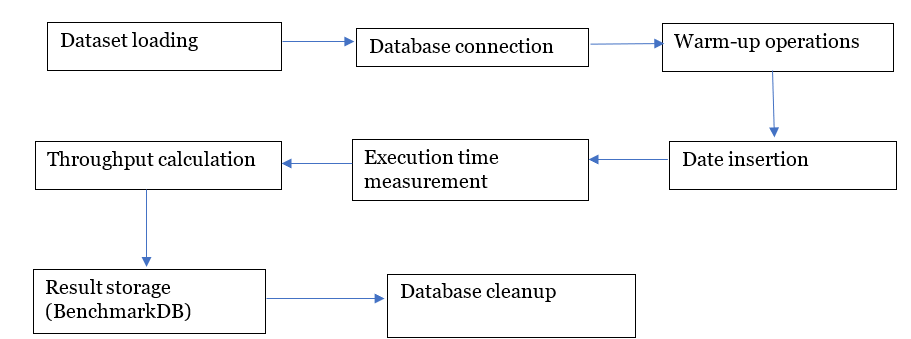
\includegraphics[width=0.8\textwidth]{figs/ingestion_benchmark_process.png}
    \caption{General Ingestion Benchmark Workflow}
    \label{fig:ingestion-benchmark-workflow}
\end{figure}

For MongoDB, benchmark datasets were loaded from JSON files. The database stored multiple observations in a single document, each representing a measurement event containing five sensor observations – salinity, conductivity, temperature, dissolved oxygen and turbidity. During execution, datasets were loaded as JSON documents. Since the datasets were defined as observations instead of documents, a conversion step was necessary to determine MongoDB batch sizes. With each document having five observations, a dataset with 1000 observations corresponded to 200 documents. After each benchmark run, all documents were removed from the collection using the cleanup functionality to prevent interference between successive executions. 


The TimescaleDB benchmark used a relational representation where each observation was stored as a single row within the observations hypertable. Datasets were parsed and converted into Observation objects just before insertion. The implementation used PostgreSQL’s bulk insertion capabilities. Observations were grouped into batches before insertion to improve efficiency and reduce transaction overhead. Insertion time was measured with nanosecond-resolution timers. After each benchmark run, the observations table was truncated to guarantee an empty database before the next insertion. 


The process was similar for InfluxDB. Benchmark datasets were converted into Observation objects with each observation getting transformed into an InfluxDB Point object. Attributes like parameters and sensor identifiers were mapped to fields and tags before getting written to the database. Batch insertion was done using InfluxDB WriteAPI that accepted collection of points and persisted them into a bucket. Similar to the other database systems, execution time measurements were collected with timers positioned immediately around the write operation. After each execution, all measurements were removed. 


In all cases, to minimize the impact of startup overheads, a warm-up strategy was used as part of the benchmarking framework. Prior to collecting performance data, each execution ran three preliminary insertion operations which were excluded from the recorded results. The warm-up executions allowed database connections to get fully established, query execution paths to get initialized and internal caches to be populated before timing began. With TimescaleDB, especially, warm-up operations reduced the influence of statement preparation and query planning overheads. For MongoDB and InfluxDB, the warm-ups helped stabilize memory allocation behavior and client-server communication. The results for the initial operations were discarded to make sure the benchmark was measuring steady-state ingestion performance. 


\section{Performance Metrics}
To make possible the comparison between InfluxDB, TimescaleDB and MongoDB, the benchmarking framework recorded a set of performance metrics for each benchmark execution. The metrics were directly calculated from the measured execution time and dataset metadata and then stored in BenchmarkDB for analysis. They include:

Execution time – This represents the total time required for the database system to finish a data insertion operation. During benchmarking, the execution time was captured using high-resolution timers. Execution time was the primary measure of ingestion performance. Lower values indicate faster loading capability. 


Throughput – Observation throughput is a measure of the number of successfully inserted observations per second. The metric normalizes ingestion performance and allows for comparison across different dataset sizes. The number of observations is the total record count per dataset while the execution time is the measured insertion time in seconds. A higher throughput indicates that the database is able to process a high number of observations per period. 



% \lstinputlisting[language=java]{code/BoksVolum.java}